\section{Response functions}\label{sec:response_functions}

The main objective of this work is to analyze the response functions. In
general we define the self- and cross-response functions in a correlated
financial market as

\begin{equation}\label{eq:response_general}
    R^{scale}_{ij}\left(\tau\right)=\left\langle r^{scale}_{i}\left(t-1,
    \tau\right) \cdot\varepsilon^{scale}_{j} \left(t\right)\right\rangle
    _{scale}
\end{equation}

where the index $i$ and $j$ correspond to stocks in the market,
$r^{scale}_{i}$ is the return of the stock $i$ in a time lag $\tau$ in the
corresponding scale and $\varepsilon^{scale}_{j}$ is the trade sign of the
stock $j$ in the corresponding scale. The subscript and superscript $scale$
refer to the time scale used, whether physical time scale or trade time scale.
Finally, we average the product over the physical time or trade time depending
on the time scale.

We use the returns and the trade signs to define three response functions:
trade time scale response, physical time scale response and activity response.

To compare the three response functions, we define the following quantities

\begin{align}
    E_{j,d}\left(t\right)&=\sum_{n=1}^{N\left(t\right)}
    \varepsilon_{j,d}^{t}\left(t,n\right)\\
    E_{j,d}\left(t\right)&=\text{sgn}\left(E_{j,d}\left(t\right)\right)
    \cdot\left|E_{j,d}\left(t\right)\right|\\
    \varepsilon_{j,d}^{p}\left(t\right)&=
    \text{sgn}\left(E_{j,d}\left(t\right)\right)
\end{align}

Where the subscript $d$ refers to the days used in the response computation.

In Sect. \ref{subsec:response_function_trade} we analyze the responses
functions in trade time scale, in Sect. \ref{subsec:response_function_physical}
we analyze the responses functions in trade time scale and in Sect.
\ref{subsec:activity_response_function} we define a response function to
analyze the influence of the frequency of trades in a second.

%%%%%%%%%%%%%%%%%%%%%%%%%%%%%%%%%%%%%%%%%%%%%%%%%%%%%%%%%%%%%%%%%%%%%%%%%%%%%%%
\subsection{Response functions in trade time scale}
\label{subsec:response_function_trade}

We define the self- and cross-response functions in trade time scale, using the
trade signs in trade time scale and the returns in physical time scale. The
response is

\begin{equation}\label{eq:response_functions_trade_scale_general}
    R^{t}_{ij}\left(\tau\right)=\left\langle r^{p}_{i}\left(t-1,\tau
    \right)\cdot\varepsilon_{j}^{t} \left(t, n\right)\right\rangle _{t}
\end{equation}

where the superscript $t$ refers to the trade time scale. However, to be
explicit with the way the averaging is made, the function reads

\begin{align}\label{eq:response_trades_explicit}
    R_{ij}^{t}\left(\tau\right)&=\frac{1}{\sum_{d=d_{0}}^{d_{f}}
    \sum_{t=t_{0}}^{t_{f}}N_{j,d} \left(t \right)} \nonumber \\
    &\cdot\sum_{d=d_{0}}^{d_{f}}\sum_{t=t_{0}}^{t_{f}}\sum_{n=1}
    ^{N\left(t\right)} r^{p}_{i,d}\left(t-1, \tau\right)\cdot
    \varepsilon_{j,d}^{t}\left(t,n\right)\\
    &=\sum_{d=d_{0}}^{d_{f}}\sum_{t=t_{0}}^{t_{f}} r^{p}_{i,d}
    \left(t-1,\tau\right) \cdot\frac{\sum_{n=1}^{N\left(t\right)}
    \varepsilon_{j,d}^{t}\left(t,n \right)} {\sum_{d=d_{0}}^{d_{f}}
    \sum_{t=t_{0}}^{t_{f}}N_{j,d}\left(t\right)} \nonumber \\
    &=\sum_{d=d_{0}}^{d_{f}}\sum_{t=t_{0}}^{t_{f}}r^{p}_{i,d}
    \left(t-1,\tau\right) \cdot \text{sgn}\left(E_{j,d}\left(t\right)\right)
    \cdot w_{j,d}^{t}\left(t\right)
\end{align}

Where

\begin{equation}\label{eq:trade_weight}
    w_{j,d}^{t}\left(t\right) = \frac{\left|E_{j,d}\left(t\right)\right|}
    {\sum_{d=d_{0}}^{d_{f}}\sum_{t=t_{0}}^{t_{f}}N_{j,d} \left(t\right)}
\end{equation}

is a weight function that depends on the normalization of the response.

To compute the response functions in trade time scale, we used all the trade
signs during a day in market time. As we can not associate an individual
midpoint price with their corresponding trade signs, all the trade signs in one
second are associated with the midpoint price of the previous second.
As $\tau$ depends on the midpoint price, even if we are using trade signs in
trade time scale, the value of $\tau$ is in seconds.

\begin{figure*}[htbp]
    \centering
    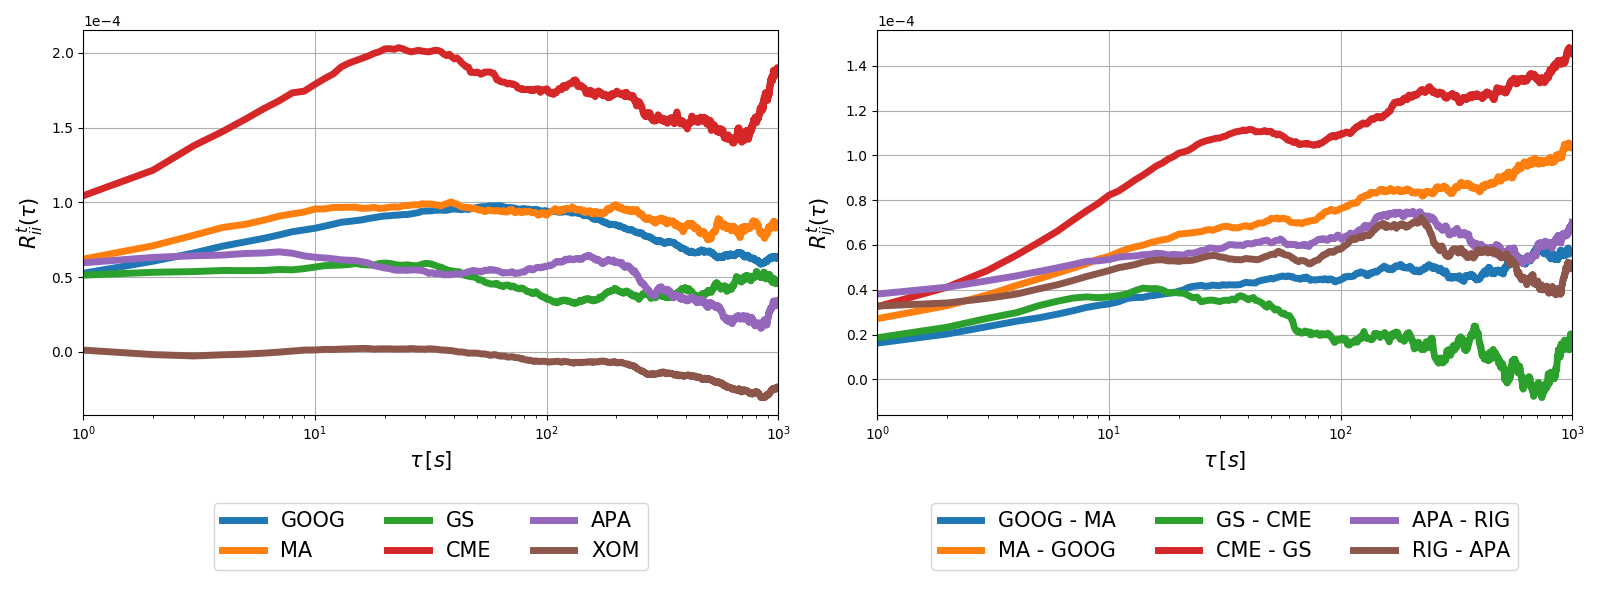
\includegraphics[width=\textwidth]
    {figures/03_responses_trade_scale_2008.png}
    \caption{Self- and cross-response functions
             $R^{t}_{ij}\left(\tau\right)$ in 2008 versus time lag $\tau$ on a
             logarithmic scale in trade time scale. Self-response functions
             (left) of individual stocks and cross-response functions (right)
             of stock pairs from the same economic sector.}
    \label{fig:response_function_trade_scale}
\end{figure*}

The results of Fig. \ref{fig:response_function_trade_scale} show the self-
responses of the six stocks used in the analysis and the cross-responses for
pairs of stocks representing three different economic sectors.

The self-response functions increase to a maximum and then slowly decrease. In
some stocks this behavior is more pronounced than in others. For our selected
tickers, a time lag of $\tau = 10^{3}$ is enough to see an increase to a maximum
followed by a decrease. Thus, the trend in the self-response functions is
eventually reversed.
On the other hand, the cross-response functions have smaller signal strength
than the self-response functions. For our cross-response functions of stocks in
the same sectors, some couples exhibit the increase-decrease behavior inside a
time lag of $\tau = 10^{3}$. Other couples seems to need a larger time lag to
reach the decrease behavior.

%%%%%%%%%%%%%%%%%%%%%%%%%%%%%%%%%%%%%%%%%%%%%%%%%%%%%%%%%%%%%%%%%%%%%%%%%%%%%%%
\subsection{Response functions in physical time scale}
\label{subsec:response_function_physical}

One important detail to compute the market response in physical time scale is
to define how the averaging of the function will be made. This, because the
response functions highly differ when we include or exclude
$\varepsilon^{p}_j \left( t\right) = 0$ \cite{Wang_2016_cross}. The
cross-responses including $\varepsilon^{p}_j \left( t\right) = 0$ are weaker
than the excluding ones due to the omission of direct influence of the lack of
trades. However, either including or excluding
$\varepsilon^{p}_j \left( t\right) = 0$ does not change the trend of price
reversion versus the time lag, but it does affect the response function
strength \cite{Wang_2016_avg}.

Regarding the definition of the response functions in- and excluding
$\varepsilon^{p}_j \left( t\right) = 0$, the general averaging is

\begin{equation}\label{eq:response_inc}
    R_{ij}^{\left(\text{inc. }0\right)}\left(\tau\right)=
    \frac{\sum_{t=1}^{T_{j}+T_{j,n}} r^{p}_{i}\left(t - 1,\tau\right)
    \cdot\varepsilon_{j}^{p}\left(t \right)}{T_{j}+T_{j,n}}
\end{equation}

\begin{equation}\label{eq:response_exc}
    R_{ij}^{\left(\text{exc. }0\right)}\left(\tau\right)=
    \frac{\sum_{t=1}^{T_{j}} r^{p}_{i}\left(t - 1,\tau\right)
    \cdot\varepsilon_{j}^{p} \left(t\right)}{T_{j}}
\end{equation}

Where the superscript inc. and exc. refers to including and excluding
$\varepsilon^{p}_j \left( t\right) = 0$. For stock $j$, $T_j$  is the total
trading time of stock $j$ and $T_{j,n}$ is the total time of lack of trading or
buy sell balance. The numerators in Eqs. \ref{eq:response_inc} and
\ref{eq:response_exc} are the same, while the denominators differ
\cite{Wang_2016_avg}.

Hence,

\begin{equation}\label{eq:relation_response_inc_exc}
    R_{ij}^{\left(\text{inc. }0\right)}\left(\tau\right)=f_{j}
    \cdot R_{ij}^{\left(\text{exc. }0\right)}\left(\tau\right)
\end{equation}

Where the relative trading frequency is defined as \cite{Wang_2016_avg}

\begin{equation}\label{eq:response_trading_frequency}
    f_{j}=\frac{T_{j}}{T_{j}+T_{j,n}}
\end{equation}

The most frequently traded stocks have $f_{i} = 1$, because the time $T_{j,n}$
is zero. According to Eq. \ref{eq:relation_response_inc_exc}, the
cross-response including $\varepsilon^{p}_j \left( t\right) = 0$ is the one
excluding $\varepsilon^{p}_j \left( t\right) = 0$ scaled by a proper
probability.

Then, we will only take in account the cross-response function excluding
$\varepsilon^{p}_j \left( t\right) = 0$.

We define the self- and cross-response functions in physical time scale, using
the trade signs and the returns in physical time scale. The response is

\begin{equation}\label{eq:response_functions_time_scale_general}
    R^{p}_{ij}\left(\tau\right)=\left\langle r^{p}_{i}\left(t-1, \tau\right)
    \cdot\varepsilon_{j}^{p} \left(t\right)
    \right\rangle _{p}
\end{equation}

where the superscript $p$ refers to the physical time scale. The corresponding
explicit expression reads

\begin{align}\label{eq:response_seconds_explicit}
    R_{ij}^{p}\left(\tau\right)&=\frac{1}{\sum_{d=d_{0}}^{d_{f}}
    \sum_{t=t_{0}}^{t_{f}} \eta\left[ \varepsilon_{j,d}^{p}
    \left(t\right)\right]} \nonumber \\
    &\cdot\sum_{d=d_{0}}^{d_{f}} \sum_{t=t_{0}}^{t_{f}}
    r^{p}_{i,d}\left(t-1,\tau\right) \cdot\varepsilon_{j,d}^{p}\left(t\right)
    \cdot\eta\left[\varepsilon_{j}^{p} \left(t\right)\right] \\
    &=\sum_{d=d_{0}}^{d_{f}}\sum_{t=t_{0}}^{t_{f}}r^{p}_{i,d}
    \left(t-1,\tau\right) \cdot\frac{\varepsilon_{j,d}^{p}\left(t\right)
    \cdot\eta\left[\varepsilon_{j,d}^{p} \left( t\right)\right]}
    {\sum_{d=d_{0}}^{d_{f}}\sum_{t=t_{0}}^{t_{f}}\eta
    \left[\varepsilon_{j,d}^{p} \left(t\right)\right]} \nonumber \\
    &=\sum_{d=d_{0}}^{d_{f}}\sum_{t=t_{0}}^{t_{f}}r^{p}_{i,d}
    \left(t-1,\tau\right) \cdot\text{sgn}\left(E_{j,d}\left(t\right)\right)
    \cdot w_{j,d}^{p}\left(t\right)
\end{align}

Where

\begin{equation}
    \eta\left(x\right)=\left\{ \begin{array}{cc}
    1, & \text{If }x\ne0 \\
    0, & \text{otherwise}
    \end{array}\right.
\end{equation}

take only in account the seconds with trades and
\begin{equation}
    w_{j,d}^{p}\left(t\right) = \frac{\eta\left[\text{sgn}
    \left(E_{j,d}\left( t\right)\right)\right]}{\sum_{d=d_{0}}^{d_{f}}
    \sum_{t=t_{0}}^{t_{f}} \eta\left[\text{sgn}\left(E_{j,d}
    \left(t\right)\right)\right]}
\end{equation}

is a weight function that depends on the normalization of the response.

\begin{figure*}[htbp]
    \centering
    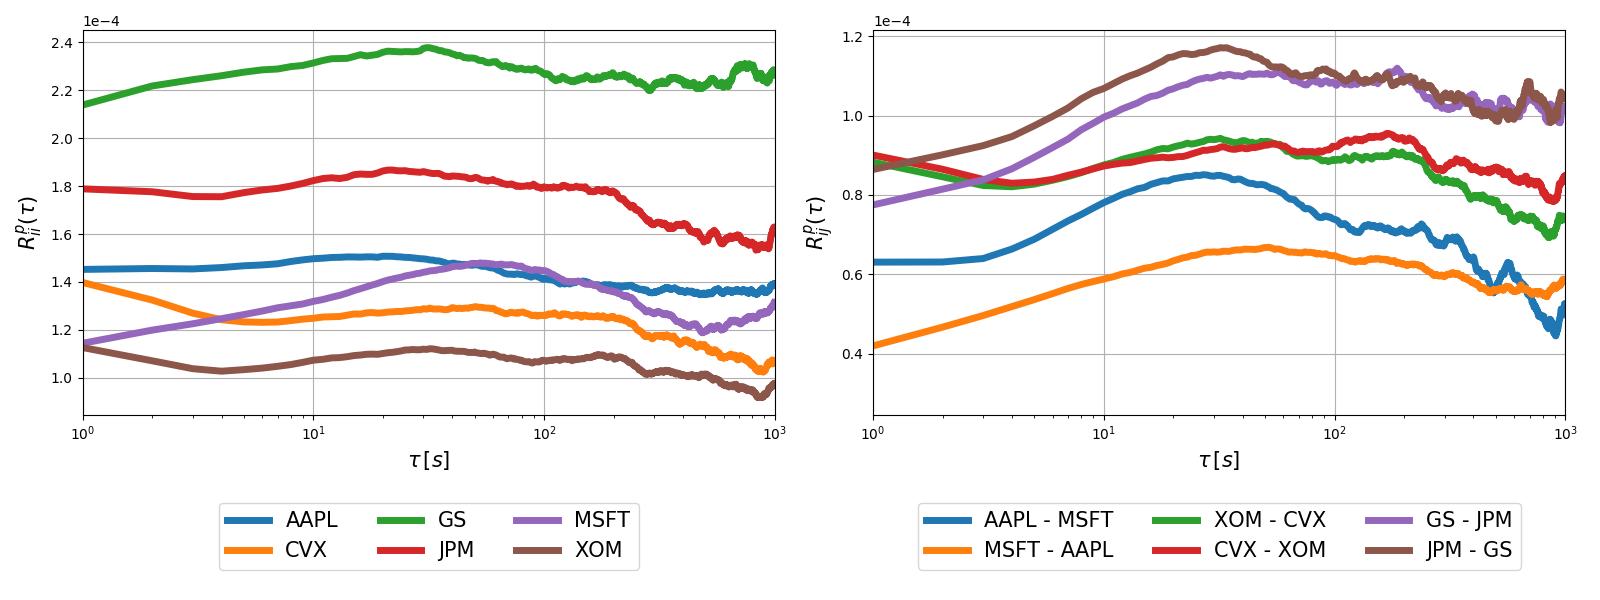
\includegraphics[width=\textwidth]
    {figures/03_responses_physical_scale_2008.png}
    \caption{Self- and cross-response functions $R^{p}_{ij}\left(\tau\right)$
             excluding $\varepsilon^{p}_{j}\left(t\right) = 0$ in 2008 versus
             time lag $\tau$ on a logarithmic scale in physical time scale.
             Self-response functions (left) of individual stocks and
             cross-response functions (right) of stock pairs from the same
             economic sector.}
    \label{fig:market_response_time_scale}
\end{figure*}

The results showed in Figure \ref{fig:market_response_time_scale} are the
self- and cross-response functions in physical time scale. For the
self-response functions we can say again that in almost all the cases, an
increase to a maximum is followed by a decrease. Thus, the trend in the self-
and cross-response is eventually reversed.
In the cross-response functions, we have a similar behavior with the previous
subsection, where the time lag in some pairs was not enough to see the decrease
of the response.

Compared with the response functions in trade time scale, the response functions
in physical time scale are stronger.

%%%%%%%%%%%%%%%%%%%%%%%%%%%%%%%%%%%%%%%%%%%%%%%%%%%%%%%%%%%%%%%%%%%%%%%%%%%%%%%
\subsection{Activity response functions in physical time scale}
\label{subsec:activity_response_function}

Finally, we define the activity self- and cross-response functions in physical
time scale, using the trade signs and the returns in physical time scale.
We add a factor $N_{j,d} \left(t \right)$ to check the influence of the
frequency of trades in a second in the response functions. The activity
response is

\begin{equation}\label{eq:activity_response_functions_general}
    R^{a}_{ij}\left(\tau\right)=\left\langle r^{p}_{i}\left(t-1, \tau\right)
    \cdot\varepsilon_{j}^{p} \left(t\right) \cdot N \left(t \right)
    \right\rangle _{p}
\end{equation}

where the superscript $a$ refers to the activity response function. The
corresponding explicit expression reads

\begin{align}
    R_{ij}^{a}\left(\tau\right)&=\frac{1}{\sum_{d=d_{0}}^{d_{f}}
    \sum_{t=t_{0}}^{t_{f}}N_{j,d} \left(t\right)} \nonumber \\
    &\cdot\sum_{d=d_{0}}^{d_{f}}\sum_{t=t_{0}}^{t_{f}}r^{p}_{i,d}
    \left(t-1,\tau\right) \cdot\varepsilon_{j,d}^{p}\left(t\right)\cdot N_{j,d}
    \left(t\right)\\
    &=\sum_{d=d_{0}}^{d_{f}} \sum_{t=t_{0}}^{t_{f}}r^{p}_{i,d}
    \left(t-1,\tau\right) \cdot\frac{\varepsilon_{j,d}^{p}\left(t \right)
    \cdot N_{j,d}\left(t\right)} {\sum_{d=d_{0}}^{d_{f}}\sum_{t=t_{0}}^{t_{f}}
    N_{j,d}\left(t \right)} \nonumber \\
    &=\sum_{d=d_{0}}^{d_{f}} \sum_{t=t_{0}}^{t_{f}}r^{p}_{i,d}
    \left(t-1,\tau\right) \cdot\text{sgn}\left(E_{j,d}\left(t\right)\right)
    \cdot w_{j,d}^{a}\left(t\right)
\end{align}

Where

\begin{equation}
    w_{j,d}^{a}\left(t\right) = \frac{N_{j,d}\left(t \right)}
    {\sum_{d=d_{0}}^{d_{f}}\sum_{t=t_{0}}^{t_{f}}N_{j,d}\left(t\right)}
\end{equation}

is a weight function that depends on the normalization of the response.

As $E_{j,d}\left(t\right)$ is the sum of $+1$ and $-1$ in one second and
$N_{j,d}\left(t\right)$ is the number of trades in a second,
$N_{j,d}\left(t\right) \ge E_{j,d}\left(t\right)$.
$N_{j,d}\left(t\right) = E_{j,d}\left(t\right)$ only when all the trades in a
second are buys $(+1)$.

The trade weight reduces noises, The physical weight gives every step the same
weight, and the activity weight emphasizes seconds with large activity.

In Figure \ref{fig:relation_responses}, we can see how the three
responses have approximately the same shape, but the strength of the signal
varies depending on the definition. The frequency of trades have a large
influence in the responses.

\begin{figure*}[htbp]
    \centering
    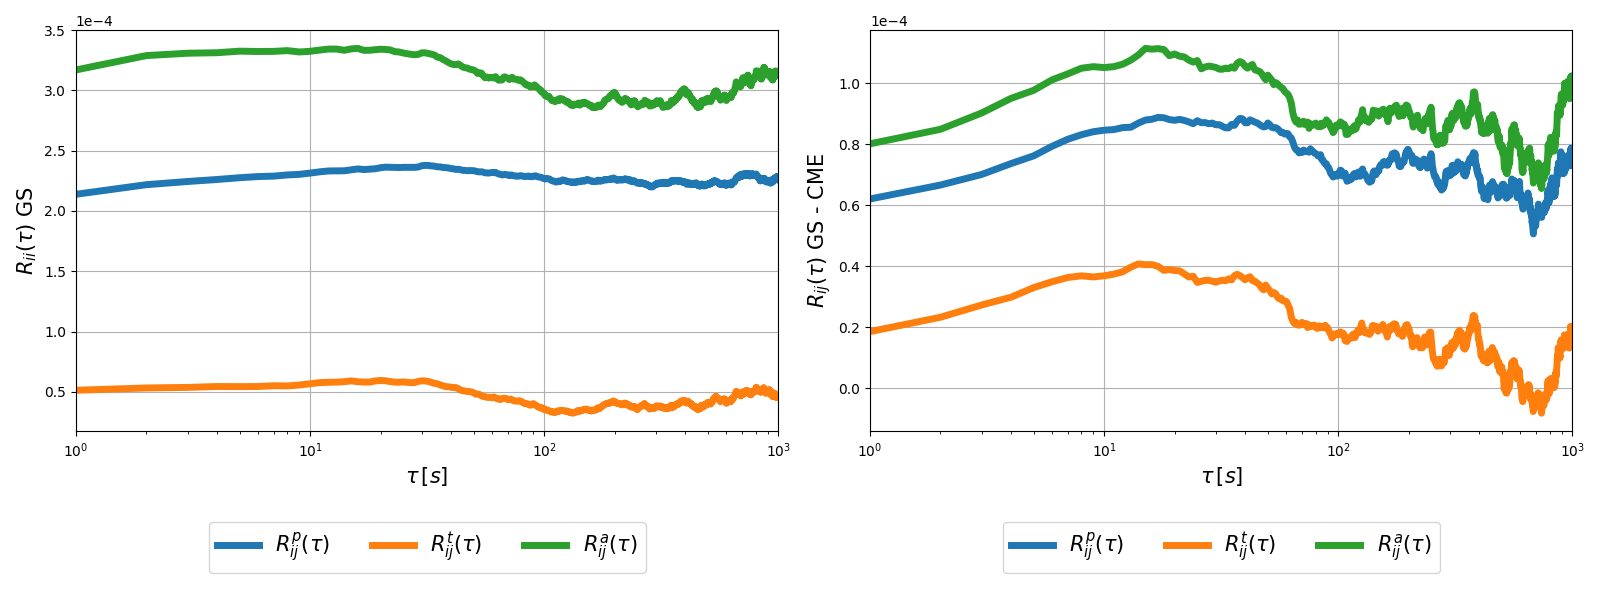
\includegraphics[width=\textwidth]
    {figures/03_response_comparison_2008_GSi_CMEj.png}
    \caption{Self- and cross-response functions
             $R^{scale}_{ij}\left(\tau\right)$ excluding
             $\varepsilon^{p}_{j}\left(t\right) = 0$ in 2008 versus time lag
             $\tau$ on a logarithmic scale. Self-response functions (left) of
             Goldman Sachs Group Inc. stock and cross-response functions
             (right) of Goldman Sachs Group Inc.-CME Group Inc. stocks.}
    \label{fig:relation_responses}
\end{figure*}

As predicted by the weights, the event response is weaker than the physical
response, and the activity response is the strongest response.

In the three curves in the figure can be seen the increase-decrease behavior of
the response functions.